% definit le type de document et ses options
\documentclass[a4paper,11pt]{article}

% des paquetages utiles classiques, en ajouter d'autres selon vos besoins
\usepackage[utf8]{inputenc}
\usepackage[T1]{fontenc}
\usepackage{amsmath}
\usepackage{amssymb,calc}
% \usepackage{fullpage}
% \usepackage{stmaryrd}
% \usepackage{url}
% \usepackage{xspace}
\usepackage[francais]{babel}

% Pour les matrices annotées ... 
\usepackage{blkarray}

% Pour les figures
\usepackage{graphicx}

% Pour les listes à puces
\usepackage{enumitem}

% \usepackage{enumerate}

\usepackage{indentfirst}

% Pour splitter la page
\usepackage{multicol}


% Évite un conflit entre french babel et enumitem
\frenchbsetup{StandardLists=true}

\usepackage[standard,framed]{ntheorem}
\usepackage{framed}

% Pour les matrices par blocs je crois ?
\makeatletter
\renewcommand*\env@matrix[1][*\c@MaxMatrixCols c]{%
  \hskip -\arraycolsep
  \let\@ifnextchar\new@ifnextchar
  \array{#1}}
\makeatother

% Pour annoter les matrices :
\usepackage{kbordermatrix} 
\renewcommand{\kbldelim}{(} % change default array delimiters to parentheses
\renewcommand{\kbrdelim}{)}


% Pour des matrices agrandies :
\newenvironment{bigmatrix}[2]{%
  \renewcommand*{\arraystretch}{#1}% 
  \begin{pmatrix}[#2]
}{%
  \end{pmatrix}
}

% Pour des commentaires à droite d'équations
\newenvironment{rcases}
  {\left.\begin{aligned}}
  {\end{aligned}\right\rbrace}

\newenvironment{lcases}
  {\left\lbrace\begin{aligned}}
  {\end{aligned}\right.}


\newcommand{\reff}[1]{(\ref{#1})}


\setlength{\parindent}{30pt}
\setlength{\parskip}{1ex}
\setlength{\textwidth}{15cm}
\setlength{\textheight}{24cm}
\setlength{\oddsidemargin}{0.2cm}
\setlength{\evensidemargin}{-.7cm}
\setlength{\topmargin}{-.5in}

% des commandes pratiques pour ecrire des maths :
\newcommand{\dx}{\,dx}
\newcommand{\dt}{\,dt}
\newcommand{\ito}{,\dotsc,}
\newcommand{\R}{\mathbb{R}}
\newcommand{\N}{\mathbb{N}}
\newcommand{\C}{\mathbb{C}}
\newcommand{\Z}{\mathbb{Z}}
\newcommand{\gO}{\mathcal{O}}
\newcommand{\Poly}[1]{\mathcal{P}_{#1}}
\newcommand{\abs}[1]{\left\lvert#1\right\rvert}
\newcommand{\norm}[1]{\left\lVert#1\right\rVert}
\newcommand{\pars}[1]{\left(#1\right)}
\newcommand{\bigpars}[1]{\bigl(#1\bigr)}
\newcommand{\set}[1]{\left\{#1\right\}}
\newcommand{\tpo}[1]{\,^t#1}
\newcommand{\derpart}[2]{\displaystyle\frac{\partial#1}{\partial #2}}
\newcommand{\der}[2]{\displaystyle\frac{\text{d}#1}{\text{d} #2}}
\newcommand{\deffonc}[3]{#1 : #2 \longrightarrow #3}
\newcommand{\Co}{\mathcal{C}}
\newcommand{\MinI}[1]{\underset{#1}{\text{Min }}}

\DeclareMathOperator{\Sup}{Sup}
\DeclareMathOperator{\Max}{Max}
\DeclareMathOperator{\Det}{Det}
\DeclareMathOperator{\diag}{diag}
\DeclareMathOperator{\Min}{Min}
\DeclareMathOperator{\Inf}{Inf}

%
%\lstset{
%  literate=%
%  {À}{{\`A}}1 {Â}{{\^A}}1 {Ç}{{\c{C}}}1%
%  {à}{{\`a}}1 {â}{{\^a}}1 {ç}{{\c{c}}}1%
%  {É}{{\'E}}1 {È}{{\`E}}1 {Ê}{{\^E}}1 {Ë}{{\"E}}1% 
%  {é}{{\'e}}1 {è}{{\`e}}1 {ê}{{\^e}}1 {ë}{{\"e}}1%
%  {Ï}{{\"I}}1 {Î}{{\^I}}1 {Ô}{{\^O}}1%
%  {ï}{{\"i}}1 {î}{{\^i}}1 {ô}{{\^o}}1%
%  {Ù}{{\`U}}1 {Û}{{\^U}}1 {Ü}{{\"U}}1%
%  {ù}{{\`u}}1 {û}{{\^u}}1 {ü}{{\"u}}1%
%}

\newlength\dlf
\newcommand\alignedbox[2]{
  % #1 = before alignment
  % #2 = after alignment
    &
    \begingroup
    \settowidth\dlf{$\displaystyle #1$}
    \addtolength\dlf{\fboxsep+\fboxrule}
    \hspace{-\dlf}
    \boxed{#1 #2}
\endgroup
}

%%%%% PACKAGE AMSTHM :
% \newtheoremstyle{definition}
%   {20pt}   % ABOVESPACE
%   {20pt}   % BELOWSPACE
%   {}  % BODYFONT
%   {0pt}       % INDENT (empty value is the same as 0pt)
%   {\bfseries} % HEADFONT
%   {.}         % HEADPUNCT
%   {5pt plus 1pt minus 1pt} % HEADSPACE
%   {}          % CUSTOM-HEAD-SPEC

\newframedtheorem{ftheo}[theorem]{Theoreme}

\theoremstyle{plain} % default
\theorembodyfont{\normalfont}
\newframedtheorem{fdef}[definition]{Définition}

\renewtheorem{remark}{Remarque}

\newframedtheorem{coroll}{Corollaire}

\newframedtheorem{prop}{Proposition}

\newtheorem{rappel}{Rappel}
\newtheorem{preuve}{Preuve}
\newtheorem{exemple}{Exemple}
\newframedtheorem{lemme}{Lemme}


\title{\huge \bfseries Optimisation sans contrainte}
\date{}
\author{}

\begin{document}
\maketitle

Étant donné $f : \R^n \longrightarrow \R$ suffisamment régulière (typiquement
$\mathcal{C}^2$), nous allons étudier d'un point de vue analytique et
numérique l'existence d'extrema de $f$ (un extremum = un minimum puis un
maximum). On parle d'optimisation \textbf{sans contrainte} (un problème 
d'optimisation avec contrainte étant posé sur un sous-ensemble de $\R^n$).
Il s'agira pour nous de trouver un \textbf{minimum} d'une fonction f, sous perte
de généralité car le maximum d'une fonction $\tilde{f}$ revient à chercher
un minimum de $f = - \tilde{f}$.

\subsubsection*{Exemples :}

\begin{enumerate}[label=-]
    \item Résolution d'un système linéaire $Ax=b$, avec $A$ symétrique définie
        positive. Exemple d'application : résolution de l'équation de Poisson
        par différences finies. Nous verrons que la solution du système
        minimise $f(x) = \frac{1}{2} \tpo{x}Ax - \tpo{b}x$. Cette propriété
        permet d'introduire de nouvelles méthodes de résolution du système.

    \item Exemple de minimisation d'une fonction non quadratique :
        \[
            \begin{array}{cc}
                f(x) = \dfrac{1}{2} \underset{1\leq i,j\leq N, i\ne j}{\sum} V(\norm{x_i - x_j}) 
                & 
                \parbox{5cm}{Cristal constitué de $N$ atomes, de positions $x_i \in \R^3$,\\ interagissent par paires via un potentiel $V$}
            \end{array}
        \]
        
        $f$ représente l'énergie potentielle totale du cristal. La forme d'équilibre du
        cristal à $T = 0$ Kelvin est donnée par un minimum de l'énergie potentielle $f$.

        Sous certaines hypothèses sur $v$ et en deux dimensions d'espace, il a été démontré
        très récemment (F. Theil, 2005) que ce minimum est atteint pour un arrangement
        périodique des atomes.
\end{enumerate}

\section{Quelques résultats de base en calcul différentiel et optimisation}

\subsection{Étude locale des fonctions à $n$ variables}

\begin{fdef}
    $f$ est différentiable en $x \in \Omega$ s'il existe une application linéaire 
    $T : \R^n \longrightarrow \R$ telle que pour $h \approx 0$ :
    \[
        f(x+h) = f(x) + T \; h + o(\norm{h})
    \]

    L'application $T$ est alors unique et on note $T = Df(x)$.

    T est appelée différentielle de $f$ au point $x$.
\end{fdef}

\begin{remark}
    Si $f$ est différentiable en $x$, alors elle est continue en $x$.
\end{remark}

\begin{lemme}
    Si $f$ est différentiable en $x$, alors $\displaystyle \frac{\partial f}{\partial x_1}(x), \dots , \displaystyle \frac{\partial f}{\partial x_n}(x)$ existent et
    $Df(x)h = \Big( \derpart{f}{x_i}, \dots \derpart{f}{x_n}(x) \Big) h$
\end{lemme}

\begin{remark}
    \begin{enumerate}
        \item Par abus de lanage, on confond souvent l'application linéaire $Df(x)$ et sa
            matrice $\Big( \derpart{f}{x_1}(x), \dots \derpart{f}{x_n}(x) \Big)$ appelée
            matrice Jacobienne de $f$ au point $x$.

        \item Le fait que $\derpart{f}{x_1} (x), \dots, \derpart{f}{x_n}(x)$ existent
            n'implique pas que $f$ est différentiable en $x$.

        \item On appelle $\nabla f(x) = \tpo{\Big( \derpart{f}{x_1}(x), \dots, \derpart{f}{x_n}(x) \Big)}$. Alors $Df(x)h = \nabla f(x) . h$ où $.$ est le produit scalaire usuel sur
            $\R^n$.
    \end{enumerate}
\end{remark}

\begin{fdef}
    $f$ est différentiable sur un ouvert $\Omega$ si elle est différentiable en tout point
    de $\Omega$.
\end{fdef}

\begin{fdef}
    $f : \Omega \longrightarrow \R$ est $\mathcal{C}^1$ si $f$ est différentiable sur
    $\Omega$ et si l'applictaion $x \mapsto \nabla f(x)$ est continue.
\end{fdef}

On peut montrer le résultat suivant :

\begin{lemme}
    $f : \Omega \longrightarrow \R$ est $\mathcal{C}^1$ si est seulement si ses dérivées
    partielles $\derpart{f}{x_i}(i=1..n)$ existent et sont continues sur $\Omega$.
\end{lemme}

\begin{fdef}
    $f : \Omega \longrightarrow \R$ est $\mathcal{C}^2$ si $f$ est $\mathcal{C}^1$ sur
    $\Omega$ et ses dérivées partielles $\derpart{f}{x_i}(i=1,\dots,n)$ sont $\mathcal{C}^1$
    sur $\Omega$.
\end{fdef}

\begin{lemme}[de Schwarz]
    Soit $f : \Omega \longrightarrow \R$ de classe $\mathcal{C}^2$. Alors pour tout $x \in
    \Omega, \forall i,j = 1..n$ : 
    \[
        \frac{\partial}{\partial x_i} \Big( \derpart{f}{x_j} \Big) (x) =
        \frac{\partial}{\partial x_j} \Big( \derpart{f}{x_i} \Big) (x)
    \]
\end{lemme}

\begin{remark}
    On notera ces dérivées $\derpart{^2f}{x_i \partial x_j}(x)$.
\end{remark}

\begin{ftheo}[formule de Taylor à l'ordre 2]
    Soit $f : \Omega \longrightarrow \R$ de classe $\mathcal{C}^2$. Pour tout $x \in \Omega$
    et $h \approx 0$ : 
\[
    f(x+h) = f(x) + \nabla f(x).h + \frac{1}{2} \tpo{h} . Hf(x) . h + o(\norm{h}^2)
\]

    avec $Hf(x) \in M_n(\R)$ définie par :
    \[
        \Big( Hf(x) \Big)_{ij} = \derpart{^2f}{x_i \partial x_j}(x)
    \]

    $Hf(x)$ est appelée matrice hessienne de $f$ en $x$ (autre notation : $H_f(x)$)
\end{ftheo}

\begin{remark}
    \begin{enumerate}[label=-]
        \item $Hf(x)$ est symétrique d'après le lemme de Schwarz.
        \item On appelle $D^2f(x)$ (différentielle seconde de $f$ en $x$) la forme
            bilinéaire symétrique $\R^n \times \R^n \longrightarrow \R$ définie par
            $D^2f(x) (h,y) = \tpo{h} Hf(x) y$.
    \end{enumerate}
\end{remark}

\begin{fdef}
    \begin{enumerate}[label=-]
        \item $f : \Omega \longrightarrow \R$ admet un minimum local en $x \in \Omega$ s'il existe
            un voisinage ouvert $u$ de $x$ tel que $f(x) \leq f(y), \forall y \in u$.

        \item $f$ admet un maximum local en $x \in \Omega$ si $f(x) \geq f(y), \forall y \in u$
    \end{enumerate}
\end{fdef}

\begin{remark}
    \begin{enumerate}[label=•]
        \item Supposons $f : \R^n \longrightarrow \R$. On parle de minimum ou maximum
            \textbf{global} lorsque $u = \R^n$.

        \item Lorsque les inégalités sont strictes (pour $y \ne x$- on parle de minimum
            ou de maximum \textbf{strict}.
    \end{enumerate}
\end{remark}

\begin{lemme}
    Soit $f : \Omega \longrightarrow \R$ de classe $\mathcal{C}^1$ ($\Omega$ \underline{ouvert} de $\R^n$). 
    
    Si $f$ admet un extremum local en $x \in \Omega$, alors $\nabla f(x) = 0$.
\end{lemme}

\begin{remark}
    \begin{enumerate}[label=-]
        \item Faux en général si $\Omega$ n'est pas un ouvert (un extremum peut être atteint
            sur le bord de $\Omega$ sans que $\nabla f$ s'y annule.

        \item $\nabla f(x) = 0$ peut être résolu par exemple par la méthode de Newton.

        \item On peut avoir $\nabla f(x) = 0$ sans que $f$ admette un extremum en $x$.
            Exemple : $f(x,y) = x^2 - y^2$ en $(x,y)= (0,0)$.
    \end{enumerate}
\end{remark}

\begin{lemme}
    Soit $f : \Omega \longrightarrow \R$ de classe $\mathcal{C}^2$. On suppose qu'il existe
    $x \in \Omega$ te que $\nabla f(x) = 0$. Alors :
    \begin{enumerate}[label=-]
        \item Si les valeurs propres de $Hf(x)$ sont $> 0$, $f$ admet un minimum local strict
            en $x$.

        \item Si les valeurs propres de $Hf(x)$ sont $< 0$, $f$ admet un maximum local
            strict en $x$.

        \item Si les valeurs propres de $Hf(x)$ sont $\ne 0$ et pas toutes de même signe,
            $f$ n'admet pas d'extremum au point $x$ ($x$ est appelé un ``point selle'').
    \end{enumerate}
\end{lemme}

\begin{remark}
    Si $Hf(x)$ n'est pas inversible, la nature du point $x$ (extremum de $f$ ou non) dépend
    des termes d'ordre supérieure donc le développement de Taylor de $f$ en $x$. Exemple :
    $f(x,y) = x^2 \pm y^2$.
\end{remark}

\begin{lemme}
    Soit $f : \Omega \longrightarrow \R$ de classe $\mathcal{C}^1$.

    Soit $x_0 \in \Omega$ tel que $\nabla f(x_0) \ne 0$. L'équation $f(x) = f(x_0)$
    définit localement (pour $x \approx x_0$) une hypersurface $S$ (de dimension $n-1$),
    qui admet un plan tangent en tout point $x \approx x_0$.

    Le plan tangent à $S$ en $x_0$ est orthogonal à $\nabla f(x_0)$.
\end{lemme}

\begin{lemme}
    Sous les hypothèses précédentes, $\nabla f(x_0)$ est orienté dans le sens
    des valeurs de $f$ croissantes. Plus précisément :
    \[
        \der{}{\varepsilon} f(x_0 + \varepsilon \; \nabla f(x_0))_{|\varepsilon=0}
        = \norm{\nabla f(x_0)}^2_2 > 0
    \]
\end{lemme}

\subsection{Conditions suffisantes pour l'existence et l'unicité d'un minimum}

Voyons d'abord une condition suffisante pour l'existence d'un minimum.

\begin{ftheo}
    Soit $\deffonc{f}{\R^n}{\R}$ continue et telle que $\underset{\norm{x} \to +\infty}{\lim} f(x) = + \infty$

    Alors il existe $x \in \R^n$ tel que $f(x) \leq f(y) \forall y \in \R^n$.
\end{ftheo}

\begin{remark}
    On dit que $f$ admet un minimum global en $x$.
\end{remark}

\begin{preuve}
    Si $\norm{y} \geq R$ avec $R$ assez grand, $f(x) \geq f(0)$.
    Donc $\underset{y \in \R^n}{\Inf f(y)} = \underset{\norm{y} \leq R}{\Inf f(y)} = f(x)$ avec $\norm{x} \leq \R$, puisque la boule $\norm{y} \leq R$ est compacte.
\end{preuve}

Le minimum de $f$ peut ne pas être unique. Nous allons donner maintenant une condition
suffisante d'unicité.

\begin{fdef}
    $\deffonc{f}{\R^n}{\R}$ est convexe si $\forall x,y \in \R^n, \forall t \in [0,1]$
    \[
        f(tx + (1-t)y) \leq tf(x) + (1-t)f(y)
    \]
\end{fdef}

\begin{remark}
    Si $\deffonc{f}{\R^n}{\R}$ est convexe, alors elle est continue sur $\R^n$.
\end{remark}

\subsubsection*{Interprétation en dimension 1 :}
\begin{figure}[h]
    \centering
    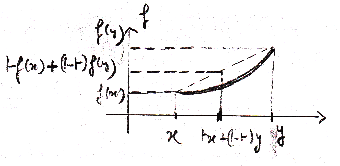
\includegraphics[scale=0.7]{7optim-dim1-convexe.png}
    \label{fig:7optim-dim1-convexe}
\end{figure}


\begin{fdef}
    $\deffonc{f}{\R^n}{\R}$ est strictement convexe si $\forall x,y \in \R^n$ tels
que $x \ne y, \forall t \in ]0,1[,$
    \[
        f(tx + (1-t)y) < tf(x) + (1-t) f(y)
    \]
\end{fdef}

\begin{ftheo}
    Si $\deffonc{f}{\R^n}{\R}$ est strictement convexe, il existe au plus un
    $x \in \R^n$ tel que $f(x) = \underset{y\in \R^n}{\Min f(y)}$.
\end{ftheo}

\begin{preuve}
    Supposons l'existene de deux minima en $x_1$ et $x_2$. Alors 
    \[
        f(tx_1 + (1-t)x_2) < tf(x_1) + (1-t) f(x_2) = f(x_1) = \underset{x \in \R^n}{\Min f(x)}
    \]

    On arrive alors à une contradiction.
\end{preuve}

\begin{remark}
    Ce théorème ne donne pas l'existence d'un minimum.

    Exemple :
\begin{figure}[h]
    \centering
    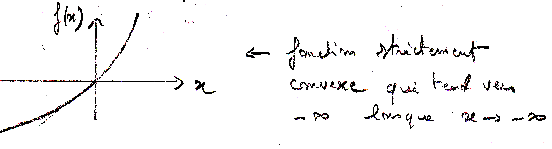
\includegraphics[scale=0.7]{7optim-min-str-cvx.png}
    \label{fig:7optim-min-str-cvx}
\end{figure}
\end{remark}

\begin{ftheo}
    Soit $\deffonc{f}{\R^n}{\R}$ strictement convexe et telle que $\underset{\norm{x} \longrightarrow +\infty}{\lim f(x)} = +\infty$. Alors il existe un unique $x \in \R^n$ tel que
    \[
        f(x) = \underset{y \in \R^n}{\Min f(y)}
    \]
\end{ftheo}

Nous allons maintenant relier les notions de point critique ($\nabla f(x) = 0$) et minimum
pour les fonctions convexes.

Le résultat suivant fournit une caractérisation utile de la convexité pour les fonctions
$\mathcal{C}^1$.

\begin{lemme}
    Soit $\deffonc{f}{\R^n}{\R}$ de classe $\mathcal{C}^1$.
    \begin{enumerate}[label=•]
        \item f est convexe si et seulement si 
            \[
                \forall x,y \in \R^n, \hspace{0.5cm} f(y) \geq f(x) + Df(x)(y-x)
            \]
        \item f est strictement convexe si et seulement si
            \[
                \forall x,y \in \R^n \text{ avec } x \ne y, \hspace{0.5cm} f(y) > f(x) + Df(x)(y-x)
            \]

            (résultat admis)
    \end{enumerate}
\end{lemme}

% Pas réussi à afficher l'image où il faut sans les vspaces ???
\vspace{0.1cm}
\subsubsection*{Interprétation en dimension 1 :}
\vspace{0.7cm}

\begin{figure}[h]
    \centering
    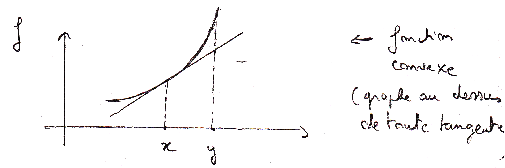
\includegraphics[scale=0.7]{7optim-cvx-tang.png}
    \label{fig:7optim-cvx-tang}
\end{figure}

\begin{ftheo}
    Soit $\deffonc{f}{\R^n}{\R}$ de classe $\mathcal{C}^1$ et convexe. Alors :
    \[
        f(x) = \underset{y \in \R^n}{\Min f(y)} \iff \nabla f(x) = 0
    \]
\end{ftheo}

\begin{preuve}
    \begin{enumerate}[label=•]
        \item ``$\implies$'' voir \S \textbf{1.1}
        \item ``$\Longleftarrow'' f(y) \geq f(x) + Df(x)\underbrace{(y-x)}_{= 0} \hspace{0.4cm} \forall y \in \R^n$
    \end{enumerate}
\end{preuve}

\begin{remark}
    On peut donc calculer numériquement les minima de fonctions convexes en recherchant
    les zéros de $x \mapsto \nabla f(x)$ (par exemple par la méthode de Newton).

    On admettra la caractérisation suivante de la convexité pour des fonctions $\Co^2$ :
\end{remark}

\begin{lemme}
    Soit $\deffonc{f}{\R^n}{\R}$ de classe $\Co^2$. Alors :

    \begin{enumerate}[label=•]
        \item $f$ est convexe $\iff \tpo{y} \; Hf(x) \; y \geq 0 \hspace{1cm} \forall x \in \R^n, \forall y \in \R^n$

        \item Si $Hf(x)$ est symétrique définie positive $\forall x \in \R^n$ alors $f$ est strictement convexe \footnotemark.
    \end{enumerate}
\end{lemme}\footnotetext{À vérifier, ce n'est pas lisible sur le kiosk}

\begin{remark}
    Pour $f(x) = \frac{x^4}{12}$ (strictement convexe), $H_f(x) = x^2$.

    $\implies H_f(0) = 0$ n'est pas symétrique définie positive.
\end{remark}

\subsubsection*{Application}
Soit $A \in M_n(\R)$ avec $A$ symétrique définie positive et $f(x)=\frac{1}{2} \tpo{x} \, A \, x - \tpo{b} \, x$

\[
    f(x) = \frac{1}{2} \sum_{i=1}^n \left( \sum_{j=1}^n a_{ij}x_j x_i \right) - \sum_{i=1}^n b_i x_i
\]

\[
    \Big( Hf \Big)_{(i,j)} = \frac{1}{2}(a_{ij} + a_{ji}) \implies
    Hf = \frac{1}{2}(A + \tpo{A}) = A \text{ (symétrique définie positive)}
\]

\[
    \implies f \text{ est strictement convexe.}
\]

De plus, $f(x) \longrightarrow +\infty$ quand $\norm{x} \longrightarrow +\infty$ car ($\lambda$ désigne
la plus petite valeur propre de $A$, qui est positive) :
\[
    f(x) \geq \frac{\lambda}{2} \norm{x}^2_2 - \norm{b}_2 \norm{x}_2 \longrightarrow +\infty \text{ quand } \norm{x}_2 \longrightarrow +\infty
\]

Donc il existe un unique $x \in \R^n \; / \; \MinI{\R^n} f = f(x)$.
Cette propriété est équivalente à $\nabla f(x) = 0$. 

\[
    \derpart{f}{x_i} = \frac{1}{2} \sum_{j=1}^n (a_{ij} + a_{ji})x_j - b_i
    \implies \nabla f(x) = \frac{1}{2}(A + \tpo{A})x - b
\]

Puisque $A$ est symétrique, $\nabla f(x) = Ax - b$. Donc :

\[
    Ax = b \iff f(x) = \MinI{\R^n} f \text{, avec } f(x) = \frac{1}{2}\tpo{x} \; A \; x - \tpo{b} x
\]

Cela permet de reformuler la résolution du système $Ax = b$ comme un problème
de minimisation.

\section{Quelques méthodes numériques pour l'optimisation sous contraintes :}

Nous abordons maintenant le calcul numérique d'un minimum de $\deffonc{f}{\R^n}{\R}$de classe $\Co^1$. On suppose que $\underset{\norm{x} \longrightarrow +\infty}{\lim} f(x) = +\infty$, de sorte que ce minimum existe.

Nous allons d'abord voir des \textbf{méthodes de gradient}, qui sont des
algorithmes itératifs utilisant uniquement $f$ et $\nabla f$.

L'exemple le plus simple d'une telle méthode est l'algorithme du
\underline{\textbf{gradient à pas constant}} :

\[
    \left\lbrace
    \begin{array}{cc}
        x_{k+1} = x_k - \rho \nabla f(x_k) & \hspace{1cm} \rho > 0 \text{ fixé} \\ [5pt]
        x_0 \in \R^n \text{ donné}
    \end{array}
    \right.
\]


Cette méthode est motivée par la propriété que $-\nabla f$ est orienté dans
le sens des valeurs de $f$ décroissantes.

On dit alors que $- \nabla f(x_k)$ est une \textbf{direction de descente} en $x_k$.

La méthode du gradient à pas constant est assez peu utilisée en pratique
car elle conduit facilement à des instabilités numériques. Par exemple,
pour $f(x) = x^4$ (fonction strictement convexe) on obtient $x_{k+1} = x_k(1-4 \rho x_k^2)$. Si $x_0^2 \geq \frac{1}{\rho}$, on montre par récurrence que
$|x_{k+1}| \geq 3 |x_k|$ (car $1-4\rho x_k^2 \leq - 3$) et donc $|x_k| \longrightarrow_{k\to +\infty} + \infty$.

Pour éviter ce type de phénomène, on peut considérer la \textbf{méthode de la
plus grande pente} (ou steepest descent method) dans laquelle $\rho$ est adapté
à chaque itération de manière \textbf{optimale} :

\[
    \begin{array}{cc}
        \left\lbrace
        \begin{array}{c}
            x_0 \in \R^n \text{ donné} \\[5pt]
            x_{k+1} = x_k - \rho_k \nabla f (x_k)
        \end{array}
        \right.
        & \hspace{1cm}
        f\left(x_k - \rho_k \nabla f(x_k)\right) = \MinI{\rho \geq 0} f \left(x_k - \rho \nabla f(x_k) \right)
    \end{array}
\]

À chaque étape de l'itération, il faut donc résoudre un problème de minimisation
en une dimension; plus précisément minimser la fonction $\deffonc{\phi}{\R^+}{\R}$ :
\[
    \rho \mapsto f(x_k - \rho \nabla f(x_k) ) := \phi (\rho)
\]
un minimum étant atteint en $\rho = \rho_k$ (le minimum existe sans être
nécessairement unique) puisque $\underset{\norm{x} \to +\infty}{\lim} f(x) = +\infty$.

\subsubsection*{Calcul de $\rho_k$ :}
Il y a plusieurs possibilités.
\begin{enumerate}[label=•]
    \item Méthode de Newton ou méthode de la sécante pour résoudre
        $\phi'(\rho) = 0$. Noter que c'est une condition nécessaire mais
        en général non suffisante pour obtenir un minimum.

        Cependant, si $f$ est convexe alors $\phi$ est aussi convexe (c'est
        la restriction de $f$ à une droite passant par $x_k$).

    Dans ce cas $\phi'(\rho) = 0 \iff \phi(\rho) = \MinI{y \in ]0,+\infty[}{\phi(y)}$

    \item Posons $a = 0$.
        
        On suppose $\deffonc{\phi}{[a,b]}{\R}$ unimodale, c.à.d. 
        \[
            \exists \rho^
        \in ]a,b[ \text{ tel que } \phi' < 0 \text{ sur } ]a,\rho^*[ \text{ et } \phi' > 0 
        \text{ sur } ]\rho^*, b[. 
        \]
        
        On pose $\delta = \dfrac{b-a}{4}, x_i = a + i\delta$.

        Selon la position relative des $f(x_i)$ ($i = 1,2,3$) on peut choisir
        $a' < b'$ tels que $f$ est unimodale sur $[a',b'] \subset [a,b]$ et
        $b' - a' = \frac{1}{2} (b - a)$. On recommence l'opération sur
        $[a',b']$ jusqu'à atteindre la précision souhaitée.


    \item \textbf{Cas particulier d'une fonction quadratique :}
        \[
            f(x) = \frac{1}{2} \tpo{x} \; A \; x - \tpo{b} \; x
        \]
    $A \in M_n(\R)$ symétrique définie positive, $b \in \R^n$.

    Notons $r_k = \nabla f(x_k) = A x_k - b \neq 0$ (sinon le min
    est déjà atteint !)

    $\phi'(\rho_k) = 0 \iff r_{k+1} . r_k = 0 \iff \underbrace{A x_k - \rho_k \: A \: r_k }_{Ax_{k+1}} - b) . r_k = 0$

    On obtient donc explicitement : 
    \[
        \rho_k = \frac{\norm{r_k}^2_2}{\tpo{r_k} \: A \: r_k}
    \]
    avec $\tpo{r_k} \: A \: r_k \neq 0$ puisque $A$ est symétrique définie
    positive.
\end{enumerate}

\begin{remark}
    En pratique le calcul de $p_k$ n'a pas besoin d'être réalisé avec
    une très grande précision.
\end{remark}

\noindent
\begin{tabular}{||c}
\begin{minipage}[c]{15cm}
        On peut montrer que la méthode de la plus grande pente converge pour toute
        condition initiale $x_0$ si $x$ est strictement convexe. La convergence
        est linéaire et peut donc être assez lente.
    \end{minipage}
\end{tabular}

\vspace{0.3cm}

\noindent
\begin{tabular}{||c}
    \begin{minipage}[c]{15cm}
        Pour avoir ue convergence plus rapide, on peut utiliser la méthode de
        Newton pour résoudre $\nabla f(x) = 0$. En particulier, si f est
        convexe on obtient ainsi forcément un minimum de $f$. Il existe par
        ailleurs des variantes moins coûteuses que Newton et efficaces, comme
        la méthode de Broyden.
    \end{minipage}
\end{tabular}

Une autre méthode beaucoup utilisée est la \textbf{méthode du gradient conjugué}.

Soit $\deffonc{f}{\R^n}{\R}$ de classe $\Co^2$, avec $f(x) \xrightarrow{\norm{x} \to +\infty} +\infty$
et $H_f(x)$ symétrique définie positive $\forall x \in \R^n$.

$f$ possède alors un minimum global strict $\overline{x} \in \R^n$. La méthode
du gradient conjugué utilise une direction de descente plus efficace que
$\nabla f(x_k)$, qui fait également appel à $\nabla f(x_{k-1})$. Nous allons
étudier cette méthode lorsque $f$ est une fonction quadratique mais elle
s'applique dans un cadre plus général.

\section{Méthode du gradient conjugé pour une fonction quadratique}

On considère $f(x) = \frac{1}{2} \tpo{x} \: A \: x - \tpo{b} \: x$ avec
$A \in M_n(\R)$ symétrique définie positive et $b \in \R^n$. Nous avons
vu que $\deffonc{f}{\R^n}{\R}$ admet un minimum global strict en $x = \overline{x}$ avec $A \overline{x} = b$.

La méthode du gradient conjugué définit une suite $(x_k)_{k\geq 0}$ qui
converge vers $\overline{x}$. Nous allons voir que la convergence se fait
en \textbf{un nombre fini d'itérations $\leq n$};  de ce point de vue,
la méthode du gradient conjugué est donc à classer parmi les méthodes
directes. Cependant, à cause des erreurs d'arrondis, cette propriété
n'est pas vérifiée en pratique (plus particulièrement pour de grands
systèmes) et la méthode est plutôt considérée comme itérative. On
contrôlera donc cet algorithme par un nombre maximal d'itérations et
par un test d'arrêt.

\subsection{Description de la méthode :}

\noindent
\begin{tabular}{||c}
    \begin{minipage}[c]{15cm}
        On notera par la suite $r_k = \nabla f(x_k) = A x_k - b$. Si
        $r_k = 0$ alors l'algorithme s'arrête ($x_k = ?$ illisible).
    \end{minipage}
\end{tabular}

\begin{enumerate}[label=\textit{\roman*})]
    \item \textbf{Initialisation :}
        On fixe $x_0 \in \R^n$.
        \begin{enumerate}[label=-]
            \item Si $x_0 = 0$ alors l'algorithme s'arrête car $x_0 = \overline{x}$.
            \item Si $x_0 \neq 0$, on calcule $x_1$ par la méthode de plus grande pente.

                On pose $\omega_0 = \nabla f(x_0)$. 
                
                $-\omega_0 =$ direction de pente pour calculer $x_1$.
                
                $x_1 = x_0 - \rho_0 \omega_0$, \hspace{0.5cm}
                $f(x_0 - \rho_0 \omega_0) = \MinI{\rho \geq 0} f(x_0 - \rho \omega_0)$

                \begin{remark}
                    Minimum explicite car minimse un polynôme de degré 2 en $\rho$.
                \end{remark}
        \end{enumerate}

    \item \textbf{Itération :}
        On suppose connus $x_k$ et $\omega_{k-1}$ ($-\omega_{k-1}$ est la direction de la pente
        utilisée pour calculer $x_k$).

        \begin{enumerate}[label=-]
            \item Si $r_k = 0$ alors l'algorithme s'arrête car $x_k = \overline{x}$.

            \item Si $r_k \neq 0$ : on pose
                \begin{align}
                    \omega_k & = r_k + \theta_k \omega_{k-1} \notag\\ 
                    \theta_k & = \frac{\tpo{r_k} (r_k - r_{k-1}}{\norm{r_{k-1}}_2^2}
                    \label{eq:iteration}
                \end{align}
                ($-\omega_k =$ direction de la descente pour calculer $x_{k+1}$)
        \end{enumerate}

        $x_{k+1} = x_k - \rho_k \omega_k, \hspace{0.5cm} f(x_k - \rho_k \omega_k) = \MinI{\rho \geq 0} f(x_k - \rho \omega_k)$

        Dans le cas présent où $f$ est quadratique, la valeur de $\rho_k$ est
        connue explicitement (voir le lemme qui suit).
\end{enumerate}

Nous allons montrer les résultats suivants : (en patriculier, $r_k \neq 0$ implique
$\omega_k \neq 0$ puisque $r_k \perp \omega_{k-1}$


\begin{lemme}
    \begin{enumerate}[label=\textit{\roman*)}]
        \item $f(x_{k+1}) = \MinI{\theta \in \R} \MinI{\rho \geq 0} f \Big[ x_k - \rho(r_k + \theta \omega_{k-1} \Big]$

        \item $\tpo{r_k} w_{k-1} = 0, 
            \hspace{0.2cm} 
            \rho_k = \dfrac{\norm{r_k}^2_2}{\tpo{\omega_k} A \omega_k}$

        \item $\tpo{\omega_k} \: A \: \omega_{k-1} = 0 \hspace{0.5cm} (w_k \text{ et }
            \omega_{k-1} \text{ sont dits ``$A$-conjugés''})$
    \end{enumerate} 

    \label{lemme1}
\end{lemme}

\begin{lemme}
    $\tpo r_k \: r_{k-1} = 0$ et (\ref{eq:iteration}) se transforme en :
    \begin{align}
        \theta_k = \frac{\norm{r_k}_2^2}{\norm{r_{k-1}}_2^2}
        \label{eq:eqlemme}
    \end{align}
    \label{lemme2}
\end{lemme}

\begin{remark}
    Les formules (\ref{eq:iteration}) et (\ref{eq:eqlemme}) sont équivalentes pour
    une fonction $f$ quadratique. Pour $f$ plus générale, (\ref{eq:iteration}) correspond
    à la méthode de Polak-Ribière et (\ref{eq:eqlemme}) à celle de Fletcher-Reeves.
    La méthode du gradient conjugué dans le cas quadratique est dûe à Hestenes et
    Steifel (1952).
\end{remark}

\subsection{Preuve du lemme \ref{lemme1}}
Nous allons montrer successivement \textit{ii}), \textit{i}) et \textit{iii}).

Tout d'abord, puisque $f(x_{k-1} - \rho_{k-1} \omega_{k-1}) = \MinI{\rho \geq 0} f(x_{k-1} - \rho \omega_{k-1})$

On a $\nabla f(x_{k-1} - \rho_{k-1} \omega_{k-1}) - \omega_{k-1} = 0$, soit
$r_k \: \omega_{k-1} = 0 \implies \text{on a montré \textit{ii}) 1\up{ère} égalité.}$

Pour $\omega = r_k + \theta \omega_{k-1}$ on a (polnyôme du second degré en $\rho$.

\begin{align*}
    f(x_k - \rho \omega & = f(x_k) - \rho \nabla f(x_k) \: \omega + \frac{1}{2} \rho^2 \tpo \omega \: H_f(x_k) \: \omega \\
    & = f(x_k) - \rho \: r_k \: \omega + \frac{1}{2} \rho^2 \tpo \omega \: A \: \omega
\end{align*}

Puisque $r_k \: \omega_{k-1} = 0$, $r_k \: \omega$ est indépendant de $\theta$ et on obtient :
\begin{align}
    f(x_k - \rho \omega) = f(x_k) - \rho \norm{r_k}^2 + \frac{1}{2} \rho^2 \tpo \omega \: A \: \omega
    \label{eq:4}
\end{align}

Le minimum de ce polynôme de degré 2 est atteint en :
\[
    \rho_{\theta} = \frac{\norm{r_k}^2_2}{\tpo \omega \: A \: \omega} \hspace{1cm}
    \text{2\up{ème} égalité de \textit{ii})}
\]

et vaut 
\[
    f(x_k - \rho_\theta \omega) = f(x_k) - \frac{1}{2} \frac{\norm{r_k}_2^4}{\tpo \omega \: A \: \omega}
\]

Pour minimiser $f(x_k - \rho_\theta \omega)$ suivant $\theta$ il faut minimiser 
$\tpo \omega \: A \: \omega$, c'est à dire $|\omega|$.
Il faut choisir pour cela $\omega = \omega_k$ tel que $\tpo \omega_k \: A \: \omega_{k-1} = 0$, ce qu'on notera $\omega_k \perp \omega_{k-1}$ :
\[
    < r_k + \theta \omega_{k-1}, r_k + \theta \omega_{k-1} = |r_k|^2 + 2 \theta <r_k, \omega_{k-1} >
    + \theta^2 |\omega_{k-1}|^2
\]

Minimum pour :
\begin{align}
    \theta = \theta_k = - \frac{<r_k, \omega_{k-1}>}{|\omega_{k-1}|^2}
    \label{l1:eq5}
\end{align}

Donc :
\begin{align}
    \omega_k = r_k - \omega_{k-1} \frac{<r_k,\omega_{k-1}>}{|w_{k-1}|^2}
    \label{l1:eq6}
\end{align}

D'où $\omega_k \perp \omega_{k-1}$. Afin de montrer le lemme \ref{lemme1}, il reste à
montrer que (\ref{l1:eq5}) correspond bien à (\ref{eq:iteration}).
D'une part :
\begin{align}
    r_k - r_{k-1} = A \: (x_k - x_{k-1}) & = - \rho_{k-1} \: A \: \omega_{k-1} \hspace{0.5cm}\text{ donc :} \notag \\
    \tpo r_k (r_k - r_{k-1}) & = - \rho_{k-1} <r_k,\omega_{k-1}>
    \label{l1:eq7}
\end{align}

D'autre part :
\begin{align*}
    |\omega_{k-1}|^2 & = (A \omega_{k-1}, \omega_{k-1}) = -\frac{1}{\rho_{k-1}}(A (x_k - x_{k-1}), \omega_{k-1}) \\
    & = -\frac{1}{\rho_{k-1}}(r_k - r_{k-1} , \omega_{k-1}) \\
    & = \frac{1}{\rho_{k-1}}(r_{k-1}, \omega_{k-1}) \hspace{2cm} \text{(car $(r_k,\omega_{k-1}) = 0$)}\\
    & = \frac{1}{\rho_{k-1}}(r_{k-1},r_{k-1}- \theta_{k-1}\omega_{k-2}) \\
    & = \frac{1}{\rho_{k-1}}\norm{r_k}^2 \hspace{2cm} \text{(car $(r_{k-1}, \omega_{k-2}) = 0$)}
\end{align*}

Donc :
\begin{align}
    \norm{r_k}^2 = \rho_{k-1} |\omega_{k-1}|^2
    \label{l1:eq8}
\end{align}

Avec (\ref{l1:eq5}), (\ref{l1:eq7}) et (\ref{l1:eq8}) on obtient donc :
\[
    \frac{\tpo r_k (r_k - r_{k-1}}{\norm{r_{k-1}^2}}  - \frac{<r_k,\omega_{k-1}>}{|\omega_{k-1}|^2} = \theta_k
\]

On obtient donc la formule (\ref{eq:eqlemme}) plus simple pour le calcul de $\theta_k$.

\subsection{Convergence de la méthode du gradient conjugué et preuve du \ref{lemme2}}

Supposons $r_k \ne 0$ pour $k = 0,\dots,n-1$ (si $r_k$ s'annule l'algorithme converge). Cela implique
$\rho_k \ne 0$ pour $k=0,\dots,n-1$.

\begin{lemme}
    Pour tout $k=1,\dots,n$ on a :
    \[
        \begin{array}{cc}
            (P_k) &
            \left\lbrace
            \begin{array}{cc}
                r_k \: \omega_q = 0 & \text{pour $q = 0,\dots,k-1$} \\
                \tpo \omega_k \: A \omega_q = 0 & \text{pour $q = 0,\dots,k-1$} \\
                r_k \: r_q = 0 & \text{pour $q = 0,\dots,k-1$} \\
            \end{array}
            \right.
        \end{array}
    \]
    \label{lemme3}
\end{lemme}

\begin{preuve}
    Par récurrence. On considère les produits scalaires 
    \[
        \left\lbrace
        \begin{array}{ccc}
            (x,y) & = & \tpo xy = x.y \\
            & \text{et} & \\
            <x,y> \: & = & \tpo x \: A \: y
        \end{array}
        \right.
    \]

    \begin{enumerate}[label=•]
        \item $P_1$ est vraie : $r_1 \: r_0 = r_1 \: \omega_0 = 0$ (condition d'optimalité de $\rho_0$)

            \[
                < \omega_1 , \omega_0 > = 0 \hspace{1cm} \text{d'après le lemme 1}
            \]

        \item Supposons $P_k$ vraie et montrons $P_{k+1} (k \leq n-1)$. On a :

            \[
                r_{k+1}.\omega_k = 0 \hspace{1cm} \text{(condition d'optimalité de $\rho_k$)}
            \]

            \begin{align*}
                r_{k+1}.\omega_q & = (Ax_{k+1} - b, \omega_q) = \left(A(x_{k+1} - x_k) + Ax_k - b, \omega_q \right) \\
                & = - \rho_k <\omega_k,\omega_q> + r_k . \omega_q \\
                & = 0 \hspace{0.5cm} \text{pour $q=0,..,k-1$ (hyp de récurrence $P_k$)}
            \end{align*}

            Donc $r_{k+1}.\omega_q = 0$ pour $q=0,..,k$.

            Par ailleurs, $r_{k+1}.r_q = r_{k+1}.(\omega_q - \theta_q \omega_{q-1})$ \hspace{0.3cm} (avec $\theta_0 := 0$ car $r_0 = \omega_0$)

            \vspace{0.4cm}
            Donc $r_{k+1}.r_q = 0$ pour $q=0,..,k$

            \vspace{0.4cm}
            Ensuite $<\omega_{k+1},\omega_k> = 0$ d'après le lemme \ref{lemme1}, et pour
            $q=0,\dots,k-1$ :
            \[
                <\omega_{k+1},\omega_q> = <r_{k+1},\omega_q> + \theta_{k+1} <\omega_k,\omega_q> = <r_{k+1},\omega_q>
            \]
            (par l'hypothèse de récurrence $P_k$)

            \vspace{0.4cm}
            $\rho_{q+1} - r_q = A(x_{q+1}-x_q) = - \rho_q \; A \; \omega_q$ amène alors :
            \begin{align*}
                <\omega_{k+1},\omega_q> & = <r_{k+1}, \omega_q> = \frac{1}{\rho_q}(r_{k+1},-r_{q+1}+r_q) \\
                & = 0
            \end{align*}
            car $0 \leq q \leq k-1$ et $(r_{k+1},r_p) = 0$ pour $p = 0,\dots,k$

            Cela prouve $P_k$ par récurrence.
    \end{enumerate}
\end{preuve}

En conclusion, la famille $(\omega_0, \dots, \omega_{n-1})$ est libre car les $\omega_i$ sont
deux à deux orthogonaux pour le produit scalaire $<x,y> = \tpo x \; A \; y$. C'est donc une
base de $\R^n$. Puisque $r_n$ est orthogonal à $\omega_0, \dots, \omega_{n-1}$, on a donc
$r_n=0$. Nous avons donc montré que $A \, x_n = b$, i.e. $x_n=??$

\begin{ftheo}
    Soit $A \in M_n(\R)$ symétrique définie positive, $b \in \R^n$ et ${f(x) = \frac{1}{2} \tpo x \: A \: x - \tpo b \: x}$.
    Alors l'algorithme du gradient conjugué définit une suite $(x_k)_{k=0,\dots,p}$ avec
    $p \leq n$ et $A \: x_p = b$. On a $f(x_p) = \MinI{x \in \R^n} f(x)$.
\end{ftheo}

\begin{remark}
    Le cas $p<n$ est exceptionnel.
\end{remark}

Enfin, nous avons montré dans le lemme \ref{lemme3} que $r_k.r_{k-1}=0$, ce qui prouve le lemme
\ref{lemme2}.

\end{document}
